\begin{figure}[htbp]
    \centering
    \subfloat[Ablation studies on different complex initialization methods with max value 6.]
    {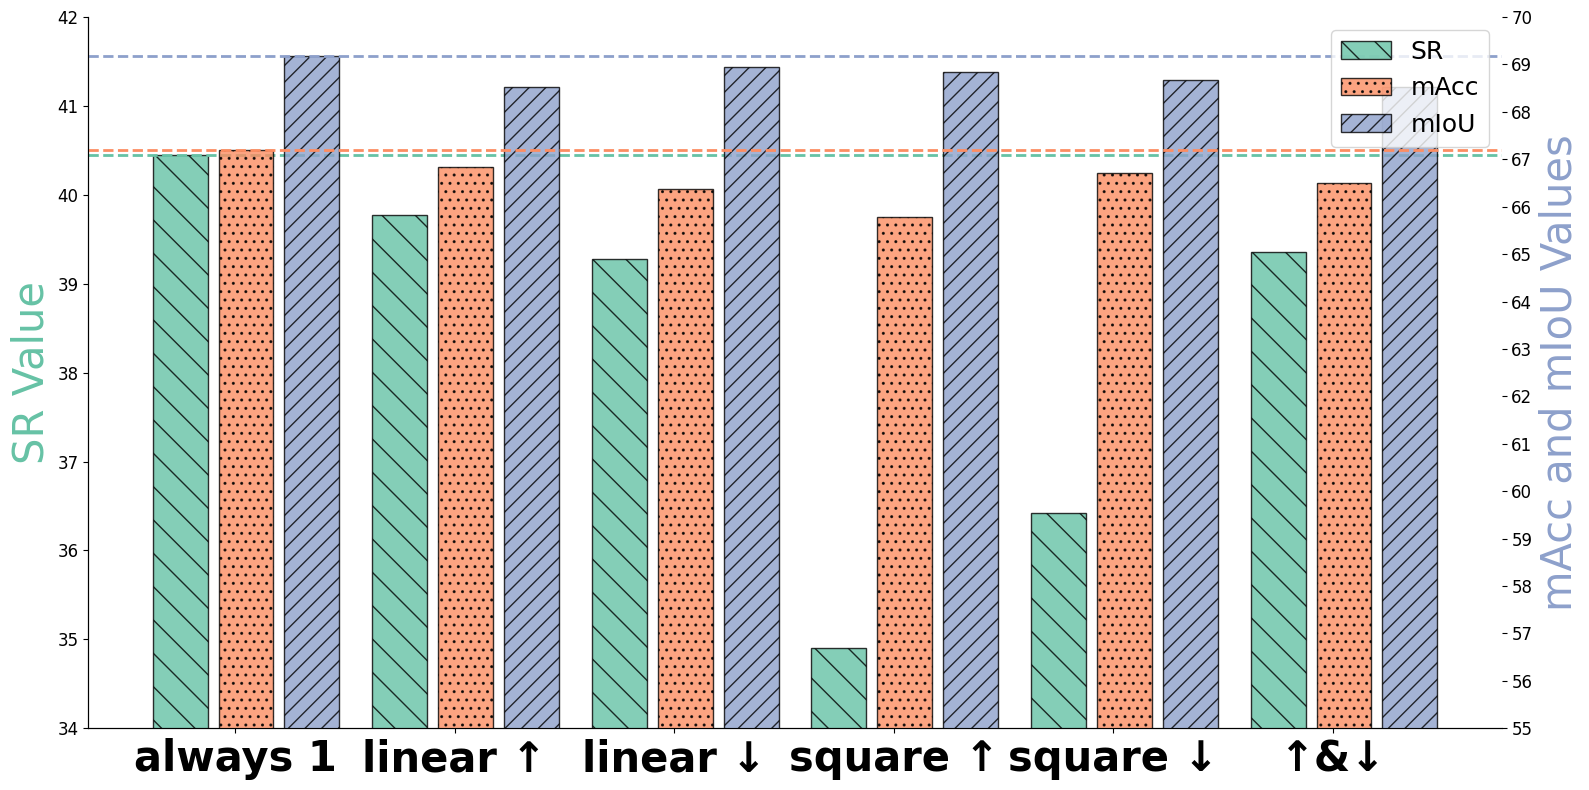
\includegraphics[width=0.45\textwidth]{figures/intx1.png}\label{fig:inxx1}}
    \hfill
    \subfloat[Ablation studies on different complex initialization methods with max value 1.]
    {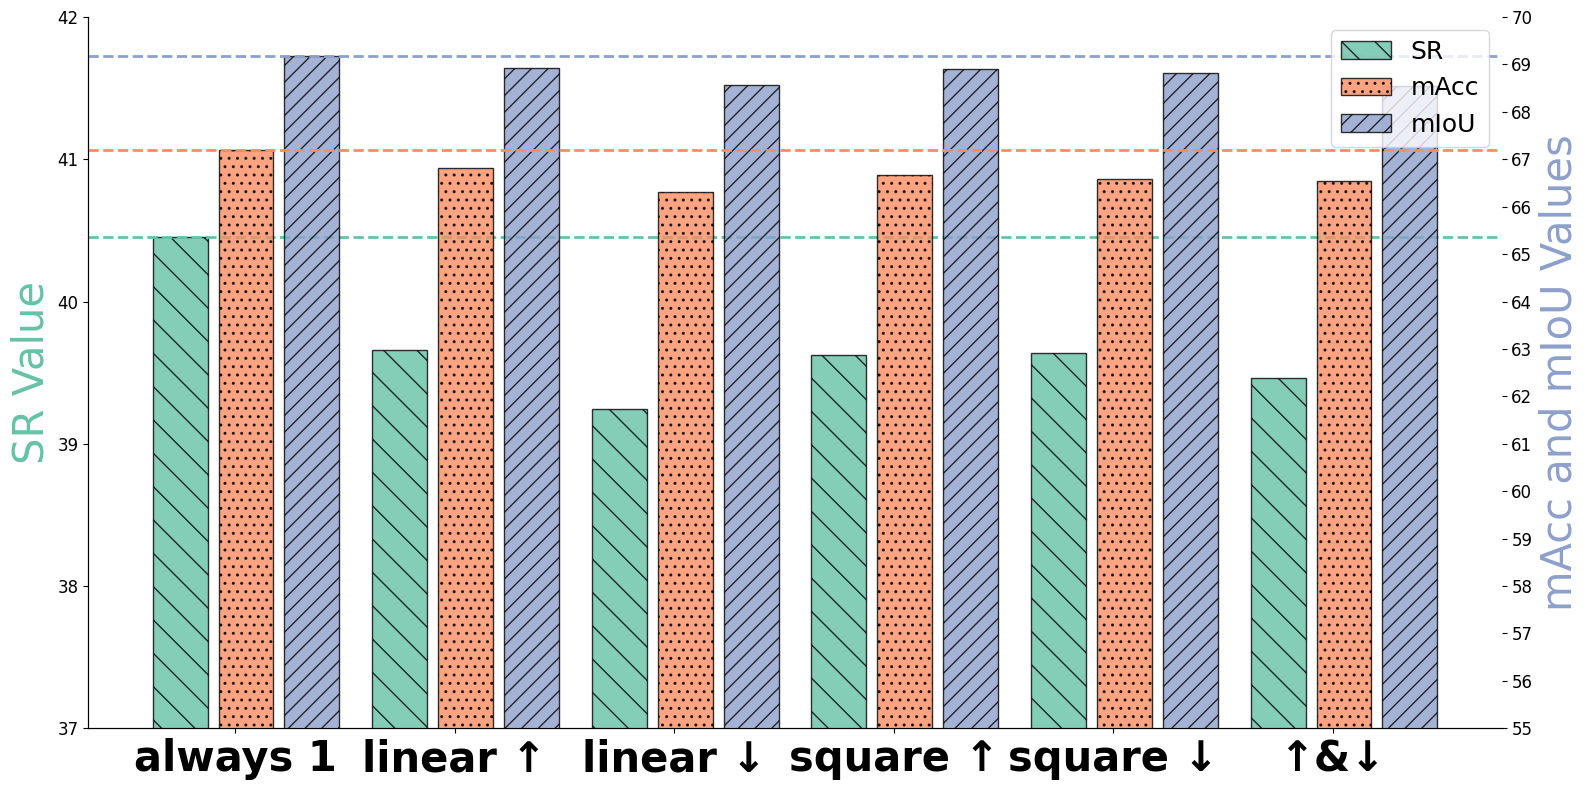
\includegraphics[width=0.45\textwidth]{figures/intx2.png}\label{fig:inxx2}}
    \caption{Ablation studies for interpolation strategy. Note: ``always 1'' indicates that $\tau$ is initialized to `1'; ``linear $\uparrow$'' denotes that the values in the matrix $\tau$ increase linearly, with the first column initialized to `1' and the last column set to `6' in \Cref{fig:inxx1}, with a gradual linear increase in between, and from `0' to `1' in \Cref{fig:inxx2}; ``linear $\downarrow$'' represents the reverse process. ``square $\uparrow$'' indicates that the value of $\tau$ increases following a square progression. ``$\uparrow$ \& $\downarrow$'' refers to a variation similar to our gradient loss weights, where the value first increases linearly and then decreases. }
    \label{fig:inxx3}
\end{figure}